\section{Modeling Data Replication and Placement}
\label{sec:model}

Our work concerns systems in which the dataset
must be partitioned among the nodes because the dataset
is too large to be completely
replicated on each node.
We replicate subsets of the whole dataset in order to increase
throughput and decrease latency.
While replication for availability is critically important, it is not a
subject of this research. 

Distributed, large-scale systems such as
Apache Hadoop, Spark, Cassandra, and Ceph
largely exploit data locality while reducing node-to-node
communication for achieving high horizontal
scaling~\cite{DeanJ2004_MapReduce,zaharia2010spark,Lakshman2010,SageWeil2006Ceph}. 
Data partitions are replicated as the system scales out.
An inefficient data placement scheme is unable to achieve the
optimal system performance and service-level objective (SLO)
violations may occur~\cite{Rodrigues2013,Cruz2013,Trushkowsky2011,Majors2010}.

The goal of this work is to place data partitions onto nodes such
that the performance is maximized for the upcoming workload.
There is a large body of work supporting workload
prediction~\cite{Gmach2007,box2015time,Akdere2012}.
This work assumes that a reliable (though not
necessarily perfect) prediction is provided by some other work.
Instead of solely relying on accurate workload prediction,
systems can dynamically adjust replication factors
and data locations for handling workload changes
~\cite{Lim2010, Trushkowsky2011, Cruz2013}.
This work focuses on determining the optimal
partition granularity, replication factors, and placement strategy.
Our work is complementary to a dynamic approach.

The following model characterizes the 
\emph{data replication and placement problem} in large-scale,
distributed systems. 
Let $M>1$ be the minimum cluster size that is sufficient to hold all
data.
The storage capacity is strictly limited by the amount of data it
physically can store locally.
In many real-world applications, $M$ is in the hundreds of nodes.
However, for this model it is only necessary that $M$ not be equal to
one, which does not require data partitioning.

Let $N$ ($N \ge M$) be the number of nodes in a cluster.
When the workload changes, the cluster expands ($N$ increases)
to meet increased demand and minimize QoS violations, or it contracts
($N$ decreases) to reduce resources and cost. 
But the cluster cannot contract smaller than the $M$ nodes needed to
hold the data.

The data is partitioned into $k \ge 1$ equal-sized data partitions on each node.
Thus, the dataset has $P = Mk$ unique partitions.
Because the cluster has $N$ nodes, there are $S = Nk$ \emph{slots} for
data partitions.
We define the \emph{replication factor}, $R$, as $R=N/M$.
When $R>1$, then $N>M$ and $S > P$ and some partitions will
be replicated among
the ``extra'' slots.
\emph{Coarse-grain} data placement occurs when there is only one
partition per node, $k=1$.
\emph{Fine-grain} data placement, $k>1$, which has more total
data partitions and partition slots, supports more distinct placements
than coarse-grain providing a better opportunity to match the
workload, and increases performance.

\medskip
\begin{tabular}[h]{lll}
  \multicolumn{3}{l}{\textbf{Model parameters}}\\
  ~~~~&\emph{Minimum number of nodes:} & $M>1$\\
  &\emph{Per node granularity:} & $k\ge 1$ \\
  &\emph{Replication factor:} & $R\ge 1$ \\
  \multicolumn{3}{l}{\textbf{Derived terms}}\\
  &\emph{Instantiated nodes:} & $N=RM$\\
  &\emph{Unique data partitions:} & $P = Mk$\\
  &\emph{Slots:} & $S = Nk = RMk$\\
\end{tabular}
\medskip

We present a motivating example below.
The base cluster has four nodes, $M=4$.
The current demand is twice the current capacity.
\myfigure{\ref{fig:dp_before_coarse}}
shows the load per partition on four nodes.
The load is unevenly distributed among the partitions.
In particular, in terms of node capacity the load on the four partitions in
\myfigure{\ref{fig:dp_before_coarse}} is 3.5, 2, 1.5, and 1 (which
conveniently totals 8).
\myfigure{\ref{fig:dp_before_fine}}, shows the same
aggregate demand as it is distributed among 16 partitions, four per
node: $k=4$.
Fine-grain replication gives rise to a \emph{placement} decision.
Redistributing loads helps reduce load imbalance among nodes
by placing highly requested partitions onto least loaded nodes.
In \myfigure{\ref{fig:dp_before_fine_placement}} the load is nearly
balanced: two nodes have a load of 2.125 and two have 1.875.
However, this alone does not help solve the overloading issue
because the workload demand is twice the system capacity.

Suppose the cluster doubles in size to eight nodes exactly meeting
anticipated demand: $R=2$ and $N=8$.
Uniform replication onto eight nodes creates two replicas of each
partition as shown in \myfigure{\ref{fig:dp_uniform}}.
The red box above the two left-most nodes shows the excess demand on those
nodes as 3.5 units of node capacity are serviced by two nodes.
The white regions in the four right-most nodes show the
underutilization because the demand is less than the capacity.

A coarse-grain, non-uniform solution is clearly better
than uniform because \emph{hotter} partitions can be
replicated more than \emph{colder} ones.
For example, in \myfigure{\ref{fig:dp_coarse}} the 3.5 units of P1 are
distributed over three nodes.
Unsurprisingly, a fine-grain solution can better match the demand to
the capacity.
\myfigure{\ref{fig:dp_fine_monochromatic}} shows that demand is perfectly matched to
capacity in this idealized example.


\myfigure{\ref{fig:dp_fine_rainbow}} shows a second placement that also
perfectly balances load but has four unique partitions on each
node.
The nodes in \myfigure{\ref{fig:dp_fine_monochromatic}} have either
one or two unique partitions.
Fewer unique partitions per node reduces the footprint of both primary
(memory) and secondary (disk) storage.
On the other hand,
more unique partitions per node increases the number of nodes that can
respond to a given request, which may better share the load among nodes.

This simple example was constructed to clearly show
the benefits of non-uniform, fine-grain data placement.
Unless the demand is uniformly distributed among the partition (an
extremely unlikely occurrence as explained in
Section~\ref{sec:workloads}) then a n\"aive uniform placement leads to
over- and underutilization.


\begin{figure}[!htbp]
\begin{subfigure}[b]{0.75\textwidth}
    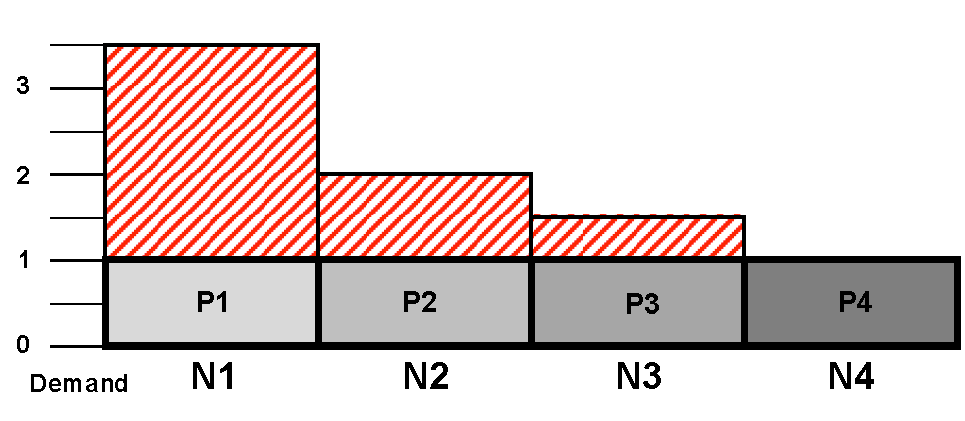
\includegraphics[width=\linewidth]{figures/dp_final_before_coarse.pdf}
    \caption{Coarse-Grain ($M=4,R=1,k=1$)}
    \label{fig:dp_before_coarse}
\end{subfigure}
\begin{subfigure}[b]{0.75\textwidth}
    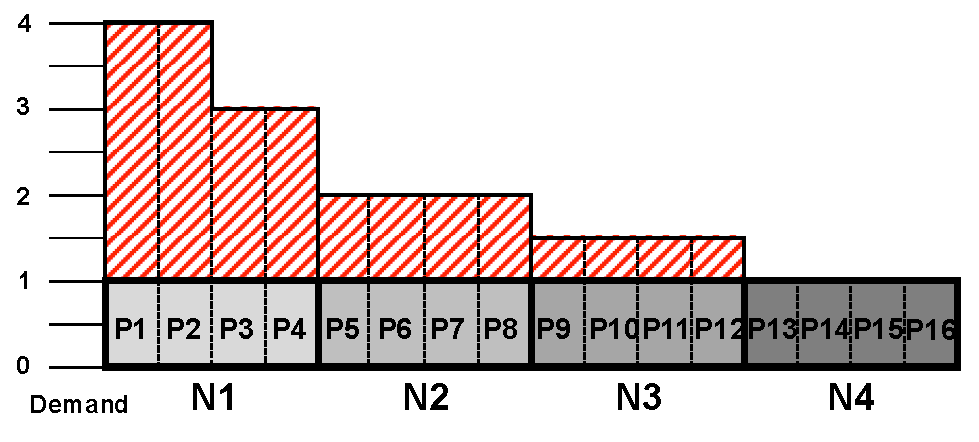
\includegraphics[width=\linewidth]{figures/dp_final_before_fine.pdf}
    \caption{Fine-Grain ($M=4,R=1,k=4$)}
    \label{fig:dp_before_fine}
\end{subfigure}
\begin{subfigure}[b]{0.75\textwidth}
    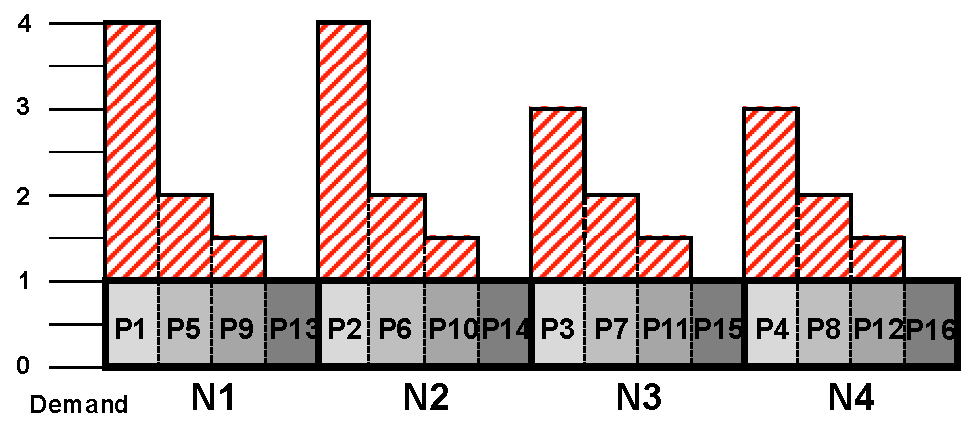
\includegraphics[width=\linewidth]{figures/dp_final_before_fine_R1.pdf}
    \caption{Fine-Grain alternative placement}
    \label{fig:dp_before_fine_placement}
\end{subfigure}
\centering
\caption{The workload demand exceeds the system capacity.}
\label{fig:dp_before}
\end{figure}


\begin{figure}[!htbp]
\begin{subfigure}[b]{0.9\textwidth}
    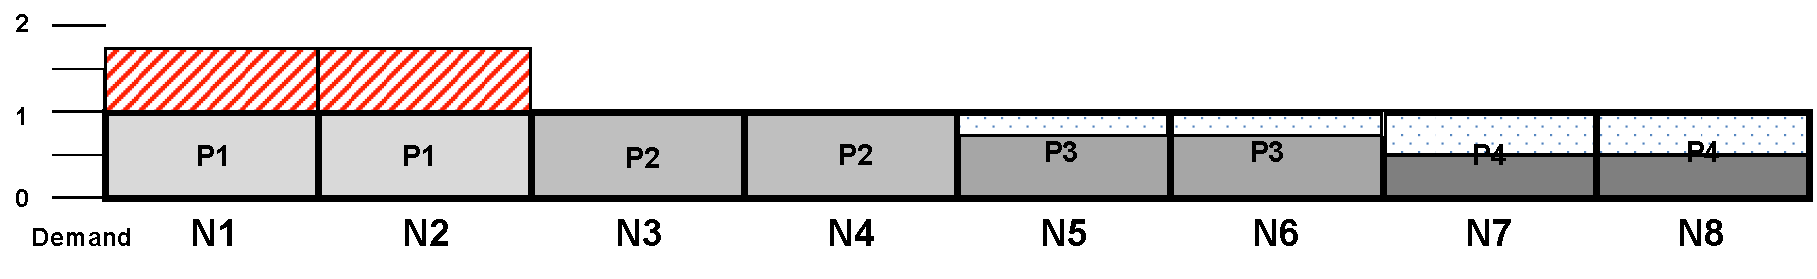
\includegraphics[width=\linewidth]{figures/dp_final_uniform.pdf}
    \caption{Uniform data placement ($M=4,R=2,k=1$)}
    \label{fig:dp_uniform}
\end{subfigure}
\hfill
\begin{subfigure}[b]{0.9\textwidth}
    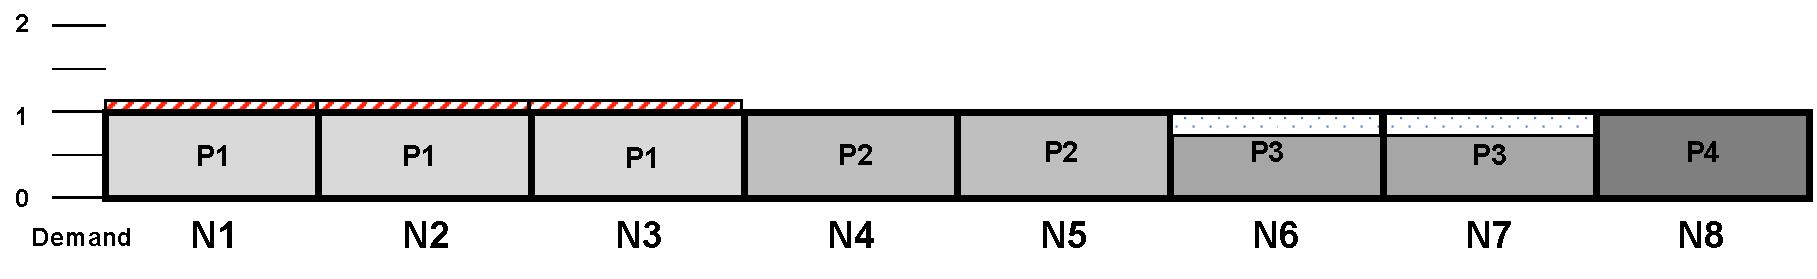
\includegraphics[width=\linewidth]{figures/dp_final_coarse.pdf}
    \caption{Coarse-grain data placement ($M=4,R=2,k=1$)}
    \label{fig:dp_coarse}
\end{subfigure}
\hfill
\begin{subfigure}[b]{0.9\textwidth}
    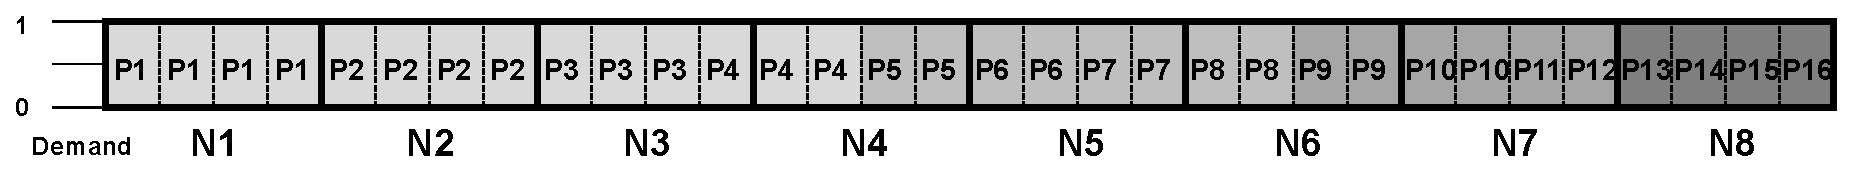
\includegraphics[width=\linewidth]{figures/dp_final_fine_monochromatic.pdf}
    \caption{Fine-grain \emph{compact} data placement ($M=4,R=2,k=4$)}
    \label{fig:dp_fine_monochromatic}
\end{subfigure}
\hfill
\begin{subfigure}[b]{0.9\textwidth}
    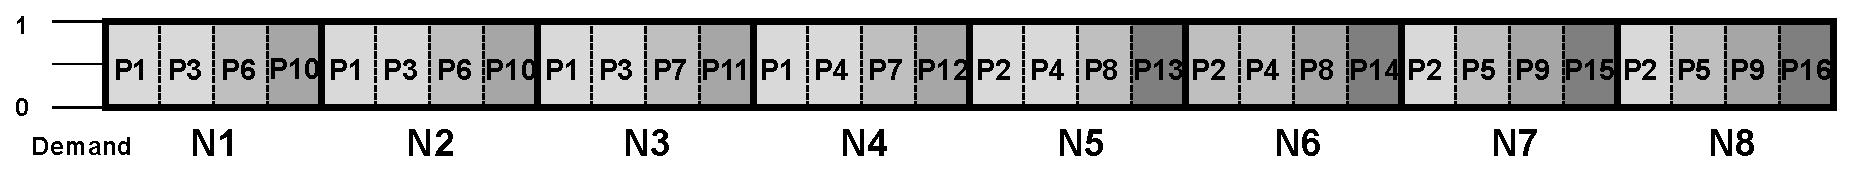
\includegraphics[width=\linewidth]{figures/dp_final_fine_rainbow.pdf}
    \caption{Fine-grain \emph{balanced} data placement ($M=4,R=2,k=4$)}
    \label{fig:dp_fine_rainbow}
\end{subfigure}
\centering
\caption{Different data placement schemes.}
\label{fig:dp_schemes}
\end{figure}
